\section{Transformée de Fourier Discrète}

\subsection{Transformée de Fourier Continue}

    Le traitement numérique du signal nécessite une discrétisation pour y appliquer des algorithmes informatiques. Avant d'aborder la transformée de Fourier discrète, il est nécessaire de définir un outil qui permet d'extraire la fréquence d'un signal. Pour une fonction $f$ représentant un signal quelconque, on utilise la définition suivante:


    Soit $f$ intégrable sur $\mathbb{R}$. La \textbf{transformée de Fourier} de $f$, notée $TF[f]$, est la fonction :
    \begin{align*}
        &TF[f] : x \mapsto \int_{-\infty}^{+\infty} f(t) \cdot e^{-2 i \pi x t}dt
    \end{align*}

    \remarque{Dans le cadre du traitement de signal, la fonction à laquelle on applique une TF est un signal, $x(t)$, sa transformée de Fourier est alors notée $X(f)$ où $f$ désigne la fréquence. On a :
    \begin{align*}
        &X(f) = \int_{-\infty}^{+\infty} x(t) \cdot e^{-i 2 \pi f t} dt \\
        &X(\omega) = \int_{-\infty}^{+\infty} x(t) \cdot e^{-i \omega t} dt \quad \text{où $\omega = 2 \pi f$, la pulsation}
    \end{align*}
    }


\subsection{Echantillonnage}

Le passage au numérique demande de ne conserver que certaines valeurs isolées du signal. Nous devons alors introduire la notion de \textbf{distribution de Dirac}. Étant donné que la définition la plus utilisée du Dirac sur $\mathbb{R}$ fait appel à des notions de théorie de la mesure et dépasse le cadre de notre étude, on présentera ici une définition plus intuitive et suffisante pour l'utilisation que l'on en fera.

Soit $(f_\alpha)_{\alpha \in \mathbb{\mathbb{R}+}}$ la famille de fonctions définies par :
\begin{align*}
    f_\alpha : t \mapsto \left\{ \begin{array}{cl} \frac{1}{2\alpha} & \text{si} \ t \in [-\alpha;\alpha] \\ 0 &  \text{sinon}
\end{array} \right.
\end{align*}

On définit l'action du Dirac $\delta$ sur une fonction $g$ continue en $0$ par :
\begin{align*}
    \int_{-\infty}^{+\infty}g(t)\delta(t)dt \coloneqq \lim_{\alpha \to 0}  \int_{-\infty}^{+\infty}g(t)f_\alpha(t)dt
\end{align*}
Soit $\alpha > 0,$
\begin{center}
    $\int_{-\infty}^{+\infty}f_\alpha(t)dt = \int_{-\alpha}^{\alpha}\frac{1}{2\alpha}dt = \frac{1}{2\alpha}\int_{-\alpha}^{\alpha}dt = 1$
\end{center}

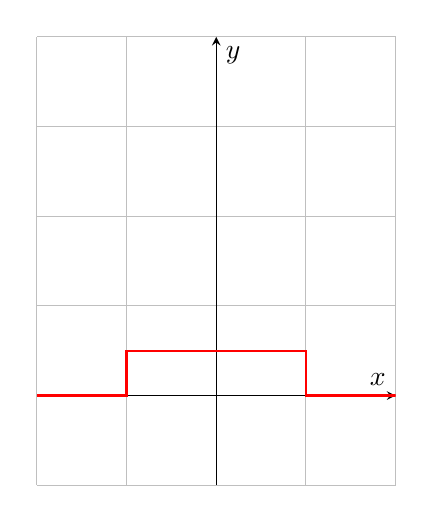
\begin{tikzpicture}[scale = 1]
\begin{axis}[
    axis lines = middle,
    unit vector ratio={1 1},
    xlabel = {$x$},
    ylabel = {$y$},
    ymin = -0.5, ymax = 2,
    xmin = -1, xmax = 1,
    grid = both,
    xticklabels = {,,},
    yticklabels = {,,},
    tick style = {draw=none}
]
\addplot [color=red, thick] coordinates {
    (-1, 0) 
    (-0.5, 0) 
    (-0.5, 0.25) 
    (0.5, 0.25) 
    (0.5, 0) 
    (1, 0)
};
\end{axis}
\end{tikzpicture}
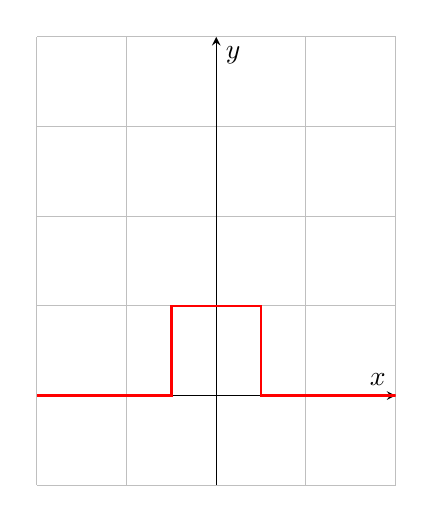
\begin{tikzpicture}[scale = 1]
\begin{axis}[
    axis lines = middle,
    unit vector ratio={1 1},
    xlabel = {$x$},
    ylabel = {$y$},
    ymin = -0.5, ymax = 2,
    xmin = -1, xmax = 1,
    grid = both,
    xticklabels = {,,},
    yticklabels = {,,},
    tick style = {draw=none}
]
\addplot [color=red, thick] coordinates {
    (-1, 0) 
    (-0.25, 0) 
    (-0.25, 0.5) 
    (0.25, 0.5) 
    (0.25, 0) 
    (1, 0)
};
\end{axis}
\end{tikzpicture}
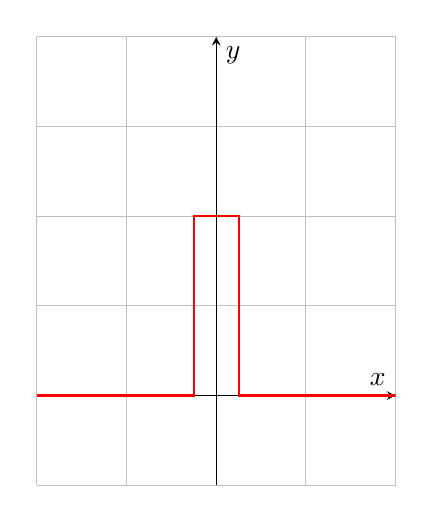
\begin{tikzpicture}[scale = 1]
\begin{axis}[
    axis lines = middle,
    unit vector ratio={1 1},
    xlabel = {$x$},
    ylabel = {$y$},
    ymin = -0.5, ymax = 2,
    xmin = -1, xmax = 1,
    grid = both,
    xticklabels = {,,},
    yticklabels = {,,},
    tick style = {draw=none}
]
\addplot [color=red, thick] coordinates {
    (-1, 0) 
    (-0.125, 0) 
    (-0.125, 1) 
    (0.125, 1) 
    (0.125, 0) 
    (1, 0)
};
\end{axis}
\end{tikzpicture}

En appliquant la définition de l'action du Dirac sur la fonction constante $g = 1$, on obtient :
\begin{align*}
    \int_{-\infty}^{+\infty} \delta(t) dt = \lim_{\alpha \to 0^+} \int_{-\infty}^{+\infty}f_\alpha(t)dt = \lim_{\alpha \to 0^+} 1 = 1
\end{align*}

En traitement du signal, on utilise souvent $\delta$ comme une fonction réelle, valant 0 partout sauf en 0 où elle vaut \og +$\infty$ \fg,  mais il s'agit bien d'une distribution caractérisée par :

\begin{description}
    \item[Sa concentration] : $\forall t \neq 0, \delta(t) = 0$
    \item[Sa masse] : $\int_{-\infty}^{+\infty}\delta(t)dt = 1$
\end{description}

On fera également attention à garder à l'esprit que la notation sous forme d'intégrale impropre sur $\mathbb{R}$ faisant intervenir le Dirac dans l'intégrande fait toujours référence à la définition de l'action du Dirac sous forme de limite et ne pose aucun problème de convergence du moment que $g$ est intégrable au voisinnage de 0.

L'intérêt, pour le traitement du signal, de la distribution de Dirac est sa capacité à isoler une valeur ponctuelle d'un signal. En effet, si on définit de la même manière, l'action du Dirac $\delta(t - t_0)$, centré en $t_0$, par l'identité $\int_{-\infty}^{+\infty} g(t) \delta(t-t_0) dt = \lim_{\alpha \to 0+} \int_{-\infty}^{+\infty} g(t) f_{\alpha}(t-t_0) dt$, alors, on obtient, pour toute fonction $g$ continue en $t_0$, la relation suivante :
\begin{align*}
    \int_{-\infty}^{+\infty} g(t) \delta(t-t_0) dt = g(t_0)
\end{align*}

\begin{proof}
    Soit $g$ une fonction continue en $t_0 \in \mathbb{R}$, on a :
    \begin{align*}
        \int_{-\infty}^{+\infty} g(t) \delta(t - t_0) dt = \lim_{\alpha \to 0+} \int_{-\infty}^{+\infty} g(t) f_{\alpha}(t - t_0) dt
    \end{align*}
    Soit $\alpha > 0$,
    \begin{align*}
        \int_{-\infty}^{+\infty} g(t) f_{\alpha}(t - t_0) dt &= \int_{t_0 - \alpha}^{t_0 + \alpha} \frac{g(t)}{2\alpha} dt \\
        &= \frac{1}{2 \alpha} \int_{t_0 - \alpha}^{t_0 + \alpha} g(t) dt \\
        &= \frac{1}{2 \alpha} \left( \int_{t_0 - \alpha}^{t_0 + \alpha} g(t_0) dt + \int_{t_0 - \alpha}^{t_0 + \alpha} \left( g(t) - g(t_0) \right) dt \right) \\
        &= g(t_0) + \frac{1}{2 \alpha} \int_{t_0 - \alpha}^{t_0 + \alpha} \left( g(t) - g(t_0) \right) dt
    \end{align*}
    Or, 
    \begin{align*}
        \left| \frac{1}{2 \alpha} \int_{t_0 - \alpha}^{t_0 + \alpha} \left( g(t) - g(t_0) \right) dt \right| &\leq \frac{1}{2 \alpha} \int_{t_0 - \alpha}^{t_0 + \alpha} \left| g(t) - g(t_0) \right| dt \\
        &\leq \sup_{t \in \left[ t_0 - \alpha ; t_0 + \alpha \right]} \left| g(t) - g(t_0) \right| \to 0 \quad \text{par continuité de g en $t_0$}
    \end{align*}

    Ainsi, on a bien $\lim_{\alpha \to 0+} \int_{-\infty}^{+\infty} g(t) f_{\alpha}(t - t_0) dt = g(t_0)$.

\end{proof}

\remarque{Cette relation s'apparente au produit de convolution $g \ast \delta$.}

Pour obtenir un échantillonnage d'un signal, il faut réaliser plusieurs extractions de valeurs à l'aide de Dirac. Il est alors pertinent d'introduire le \textbf{peigne de Dirac} de période $T$, noté $\Sha_{T}$ :
\begin{align*}
    \Sha_{T}(t) = \sum_{n\in\mathbb{Z}} \delta(t - nT)
\end{align*}

\begin{center}
    \begin{tikzpicture}[scale=1.5]

    \draw[->] (-3,0) -- (3,0) node[right] {$t$};
    \draw[->] (0,-0.5) -- (0,1.5) node[above] {$\Sha_{T}(t)$};

    \foreach \x in {-2.5, -2, ..., 2.5} {
        \draw[-, blue, thick] (\x, 0) -- (\x, 1);
        \draw[dashed, blue, thick] (\x, 1) -- (\x, 1.5);
    }
    \draw[<->] (1, -0.2) -- (1.5, -0.2) node[midway, below, font=\tiny] {$T$};
\end{tikzpicture}
\end{center}

Le signal échantillonné $s_e(t)$ est alors modélisé par le produit du signal analogique $s(t)$ et du peigne de Dirac $\Sha_{T}$:
\begin{align*}
    s_e(t) = s(t) \cdot \Sha_{T}(t) = \sum_{n\in\mathbb{Z}} s(nT) \delta(t - nT)
\end{align*}

Cette expression transforme une fonction continue en une suite de coefficients $s(nT)$ qui pourront être traités avec des méthodes numériques.

\begin{center}
    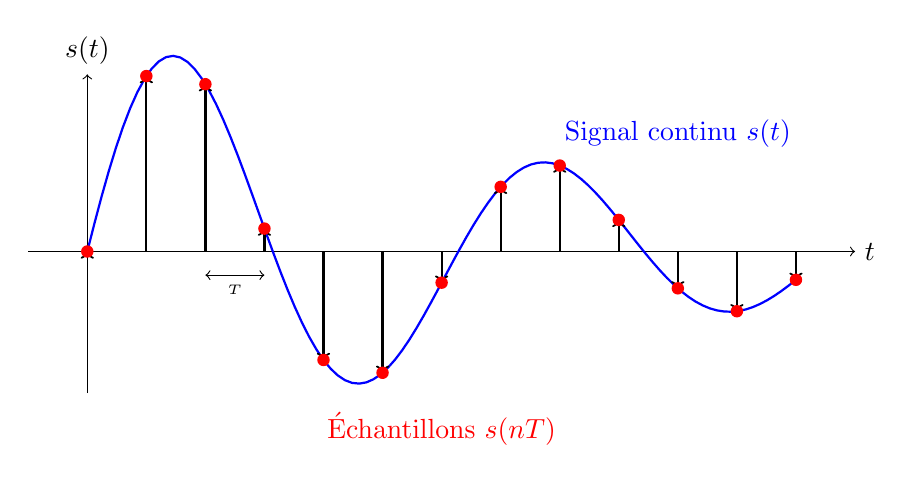
\begin{tikzpicture}[scale=1.5]

    \draw[->] (-0.5,0) -- (6.5,0) node[right] {$t$};
    \draw[->] (0,-1.2) -- (0,1.5) node[above] {$s(t)$};

    \draw[thick, blue, domain=0:6, samples=100] 
        plot (\x, {2*exp(-\x/4)*sin(2*\x r)});
    \node[blue] at (5,1) {Signal continu $s(t)$};

    \foreach \x in {0, 0.5, ..., 6} {
        \pgfmathsetmacro{\y}{2*exp(-\x/4)*sin(2*\x r)}
        \draw[->, black, thick] (\x, 0) -- (\x, \y);
        \fill[red] (\x, \y) circle (1.5pt);
    }
    \node[red] at (3,-1.5) {Échantillons $s(n T)$};
    \draw[<->] (1, -0.2) -- (1.5, -0.2) node[midway, below, font=\tiny] {$T$};
\end{tikzpicture}
\end{center}